\chapter{Overview}

The result of this research was the development of |miq|, a package manager and
build system for Linux.

miq is a single-file executable that handles the full lifecycle of the build
process of the packages it manages. This stages include:

\begin{enumerate}
    \item Evaluating the expressions that describe packages
    \item Calculating the dependency graph
    \item Fetching the necessary source code
    \item Performing the described build process
    \item Handling the storage and tracking of the installed packages
\end{enumerate}

Therefore, the following sections will all the components that make up miq, and
their interactions.

\section{Unique identifiers}

The development of miq aimed for a modular design, such that
each component didn't have much coupling with the others.
This allows for easy refactoring of parts of the source
code, while leaving the rest of the system untouched. As
such the components of miq can be layed out in figure
\ref{fig:miq-components} .

\begin{figure}[hbtp]
    \centerfloat
    % 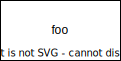
\includegraphics{assets/overview.png}
    \includesvg[width = 450pt]{assets/overview.svg}
    \caption{Overview of the subsystems of miq}
    \label{fig:miq-components}
\end{figure}

Miq is presented as a pipeline of stages, where each
subsystem transform the input data to achieve a desired
state. This design is inspired by other package managers,
which present a similar structure of stages. The main
difference, is that miq works on static package definitions
layed out in a file, which describe the desired state of the
system. In contrast to other package managers, like |apt|,
where the final state of the system is a succession of
commands executed in the shell.

On of the main differences of miq to other package managers,
is how the files are layed out in the filesystem. This is
because each package is given a unique identifier, which in
turns is used for the directory where the package will be
located. This identifier is also unique between different
versions of the same package. And not only that, but it also
encodes the recipe used to build the package itself, and all
of its parents.

To accomplish the tagging of each package with an unique
identifier, a flow of data from package input to package is
visualized on figure \ref{fig:hash}. From a |PackageInput|,
a unique hash is generated, that is the result from hashing
all the fields of the struct. Finally, the hash (an unsigned
32-bit integer) is encoded into text, to form the name of
the package. For this application, the algorithm used is the
\textit{Fowler-Noll-Vo} hash function, which is implemented
in the |fnv| create \cite{FnvRust} . This hash function is
not cryptographically secure, but this was not one of the
design requirements of miq (and can be swapped out for any
other hashing algorithm as needed, as long as it conforms to
the |Hash| trait in Rust).



\begin{minted}{rust}
#[derive(Hash)]
struct PackageInput {
    name: String,
    version: Option<String>,
    script: MetaTextInput,
    deps: Option<Vec<Unit>>,
    env: Option<BTreeMap<String, MetaTextInput>>,
}
\end{minted}

\begin{figure}[hbtp]
    \centerfloat
    \includesvg[width = 0.7\paperwidth ]{assets/hash.svg}
    \caption{Overview of the hashing algorithm}
    \label{fig:hash}
\end{figure}

The implications of this design is that any package gets a
different place on the filesystem, which is derived from
everything that defines the package itself - its build
script and its dependencies, which in turn are also hashed
by the same rules. The advantage of this design, is that
every package has its dependencies perfectly defined,
instead of relying on automatic detection. Let's say that
package |foo| depends of package |bar|. On a conventional
package manager, if |bar| is changed in any form (for
example, updated), then |foo| is usually not modified. But
in essence, now |foo|, if we consider it as a whole, that is
its whole dependency tree, it has changed. This poses a big
issue for the reproducibility of an operating system. Is
|foo| the same if we swapped |bar| for a different version?
Or if we swapped one of |bar|'s dependencies? (Figure
\ref{fig:depswap}) In miq, it is clear that the packages are
no longer the same, as the hashes of its entire dependency
tree has changed, and therefore the name of the output
package. This means that a package "foo" does not really
exist in miq, but rather a package "foo" with a specific hash.

\begin{figure}[hbtp]
    \centerfloat
    \includesvg[width = 200pt]{assets/depswap.svg}
    \caption{Change of dependencies for a package for a conventional package manager}
    \label{fig:depswap}
\end{figure}

% insert depswap-miq.svg
\begin{figure}[hbtp]
    \centerfloat
    \includesvg[width = 200pt]{assets/depswap_miq.svg}
    \caption{Change of dependencies for a package for miq}
    \label{fig:depswap_miq}
\end{figure}

\FloatBarrier
\section{Graph-based dependency resolution}

In software deployment, one of the main goals is to have be
able to reproduce a deployment environment as reliably as
possible. This means that any external factors should be
reduced to a minimum, such that the end result is as close
to the expected as possible. The reality of system
deployments is that not all environments are the same, such
that the same deployment can be applied to different systems
with different hardware -- for example, different network
cards, hard drives or even different architectures.

On the software side, the same problem exists. Any
deployment is composed of different parts of software which
interact with each other. To reduce any external factors,
a possible solution is to try to control the entire software
stack -- from the kernel, to the operating system and
libraries and finally to the application to be deployed.
This can be seen in the deployment of an entire \ac{VM}, that
contain the specific OS required for the application. But
this is not always possible, for example in a managed
environment from a cloud provider. Or it may not be desired
for the cost of implementation and maintenance. One of the
most popular solution nowadays is the use of containers
\cite{DockerAcceleratedContainerized2022}. A container is a
collection of files packaged into an \textit{image}, which is
run by a \textit{container runtime}. The runtime is able to
isolate the main process of the container by using special
Linux capabilities, such as \textit{namespaces}
\cite{NamespacesLinuxManualb}. By isolating the ``child''
process from the host, the container is able to bundle its
entire dependency tree without conflicts with the host.

What is proposed in this project is the usage of the hashing
techniques discussed in the previous section to achieve
isolation of the dependency tree of a child process from the
host. Each file which lives in the miq store, has a unique
path according to its hash.

\begin{minted}{text}
gcc-e3591c92b6d130e5        =>  /miq/store/gcc-e3591c92b6d130e5
bootstrap-5f87f2800c8c639e  =>  /miq/store/bootstrap-5f87f2800c8c639e
\end{minted}

For this reason, a runtime to isolate a process (what is
done with containers) is not needed. Instead, each process
can directly reference the absolute path to the exact
dependency in the store. If package A requires dependency B,
it does not matter if the host \ac{OS} uses also B. If it is
a different version, it will be reflected on its hash -- and
path. If it is exactly the same package B, then the
dependency will be able to be shared across the applications.

\begin{figure}[hbtp]
    \centerfloat
    \includesvg[width=250pt]{assets/depshare.svg}
    \caption{Dependency sharing between applications.}
    \label{fig:dep_share}
\end{figure}

As figure \ref{fig:dep_share} shows, if a there is a
dependency A which is used by two applications, if A is not
the same, the will be no conflict in the file system, as it
will use a different path. By using this technique, we are
able to share the dependencies of multiple application
without the need for containers or namespaces, towards a
more ``native'' approach.

\begin{minted}{text}
identifier => id+hash          => path
A-1.0.0    => A-1.0.0-1f0d1c2b => /miq/store/A-1.0.0-1f0d1c2b
A-1.0.1    => A-1.0.1-a2b3c4d5 => /miq/store/A-1.0.1-a2b3c4d5
A-2.0.0    => A-2.0.0-1f0d1c2b => /miq/store/A-2.0.0-1f0d1c2b
\end{minted}

For the sake of simplicity, the result hash is stripped of
identifiers. Internally, these hashes would be tracked by
the package manager. But for the representation of the
dependency graphs, they are assumed to be computed by miq,
but not displayed. As said in previous sections, the design
decision of tracking each package with a unique hash,
implies that when a node is displayed with a name ``A'', it
is a unique package based on its dependencies and definition
of the package itself.

The data structure used to represent the dependency graph of
a given node ``N'', is a \acl{DAG}. A directed graph
consists of a non-empty finite set of elements called nodes
and a finite set of ordered pairs of distinct nodes called
edges. A directed graph with no cycles is called a \ac{DAG}
\cite{bang-jensenDigraphs2009} . The representation of this
is simply a list of nodes and edges such as the following.

\begin{figure}[hbtp]
    \centering
    \begin{minipage}[t]{0.5\textwidth}

    \begin{minted}{dot}
        digraph G {
          // Nodes
          a;
          b;
          c;
          // Edges
          a -> b;
          a -> c;
          b -> c;
        }
    \end{minted}
    \end{minipage}
   \caption{\texttt{dot} language for describing graphs.}
   \label{fig:dot_graph}
\end{figure}

\begin{figure}[hbtp]
    \centerfloat
    \includesvg[width=70pt]{graph/sample.dot.svg}
    \caption{Resulting visualization for the graph in figure \ref{fig:dot_graph}.}
\end{figure}

For a generic \ac{DAG}, we can define the nodes and edges as
``weighted''. A weight is a value attached to the element.
Common examples of weighted nodes are ``labels'' -- like
|a,b,c| in figure \ref{fig:dot_graph} -- numeric values,
that can represent a cost or a distance, depending on the
application of the graph. Edges can also be weighted, with
also the common use of numeric values. For the topic of
package management, on first instance the edges are not
weighted -- or implemented as a |null| value. The nodes then
can represent an identifier for a package. Because in the
miq software deployment model, we can identify a package by
its path in the store
(|/miq/store/<name>-<version>-<hash>|), a node weight can be
represented just by a |String| type in Rust. Therefore, the
edge directions represent a dependency between two packages,
read like:

\begin{minted}{text}
"A depends on B"
 A    ==>     B
\end{minted}

For the purpose of this application, the term "to depend on"
is flattened over any type of dependency. Instead of
specifying whether a dependency occurs at ``runtime'' or
``buildtime'', this is simplified to just ``depend''. An
example of how dependencies can be split into different
categories is present in \textit{Gentoo's Ebuild system}
\cite{DependenciesGentooDevelopment}. In Gentoo,
dependencies are split in 3 categories: |BDEPEND| (required
at build-time in the build machine), |DEPEND| (required at
build-time, for the target machine) and |RDEPEND| (required
at run-time, for the target machine) (figure \ref{fig:dep_categories} ). Many Linux
distributions implement the same 3 variants, with different
naming conventions. What this allows it stripping packages
once the package has been built. This is specially useful on
binary-based distributions, where you don't need to
distribute the compiler for a package, but only its
link-time dependencies and run-time dependencies. As noted
before, these differences are not considered in miq, and
just a generic ``dependency'' is used for both run-time and build-time.

\begin{figure}[hbtp]
    \centerfloat
    \begin{tabular}{lll}
        \hline
        & Build-time & Run-time \\
        \hline
        Build machine & |BDEPEND| & - \\
        Target machine & |DEPEND| & |RDEPEND| \\
        \hline
    \end{tabular}
    \caption{Dependency categories in Gentoo \cite{DependenciesGentooDevelopment} .}
    \label{fig:dep_categories}
\end{figure}

Finally, one of the properties of a \ac{DAG} is that there
is always an acyclic ordering of the nodes
\cite{bang-jensenDigraphs2009}. This means, that we can get
an ordered list of all the nodes starting from a root node,
without cycles. A cycle in package management is an
undesirable entity. What it is translated to, is that ``a
package depends on itself''. For a binary based
distribution, this is not a hard problem to solve, as the
packages are usually applied into the system in any order.
But for a source-based distribution, a cycle in the
dependency graph is impossible to solve: to be able to build
a package, we require the package itself as an input,
leading to a paradox. This is usually solved by introducing
multiple ``intermediate'' packages -- for example, a package
A without less features, such that it doesn't depend on
itself.

The usage of a \ac{DAG} is also very useful to represent the
dependencies in a manifest on disk. As instead of committing
multiple actions into the live system, a manifest can be
used to declare all dependencies front-loaded.

In the following sections, it is described how the dependency
graphs are implemented in miq, and how they are used to walk
the dependency tree to build all packages in parallel.

\begin{figure}[hbtp]
    \centerfloat
    \includesvg[width=0.7\paperwidth]{graph/libc.dot.svg}
    \caption{Dependency graph for the package
    \texttt{stage0.libc}, hashes stripped.}
    \label{fig:m4_graph}
\end{figure}

\subsection{Immutability}

To build reliable system deployments, it is important to reduce the
number of variables that can affect the outcome. From the
software perspective, this means that the system should
either be reliant to changes in the environment, or minimize
the factors from the host that can affect the application.
In Linux, one of the main factors that can affect the
environment are the libraries that are installed on the
system.

On the previous section it was discussed how a different
approach to tagging the packages on the filesystem can be
used to achieve a consistent environment. What this
filesystem layout naturally leads into, is a system where
there is no mutation of the existing packages. On a
classical system, to upgrade a package, the following steps
are taken:

\begin{enumerate}
    \item Download the new update for package |foo|, and unpack it
    \item Replace file |/usr/bin/foo| with the new version
    \item Replace file |/usr/share/foo-bar| with the new version
    \item \ldots
    \item Register the new version in the database
\end{enumerate}

As can be seen, the process of upgrading a package involves
multiple in-place modifications of the existing package.
This operation can be qualified as ``surgical'', as it may
involve many operations which can fail -- and always
eventually fail. A failure in the middle of a upgrade
process can leave the system on a inconsistent state.

\begin{enumerate}
    \item Download the new update for package |foo|, and unpack it
    \item Replace file |/usr/bin/foo| with the new version
    \item Failed to upgrade |/usr/share/foo-bar|, aborting
\end{enumerate}


\subsection{Atomicity}

\FloatBarrier
\section{ELF format}
\label{sec:elf-format}

Once decided to use this technique for tagging packages, by
using the hash of the package's build script and
dependencies, they key aspect to understand is how this
translate into the underlying file format using by Linux:
ELF. It stands for \textit{Executable and Linkable Format}.
This file format is used both in Linux and the BSD family of
operating systems, and consists of header and symbol tables,
that wrap the underlying assembly to be executed by the
processor \cite{LinuxFoundationReferenced}. The ELF format
is used by any CPU architecture that Linux supports, so the
ELF format is just a ``container'' for the assembly that is
to be executed.

\begin{figure}[hbt]
    \centerfloat
    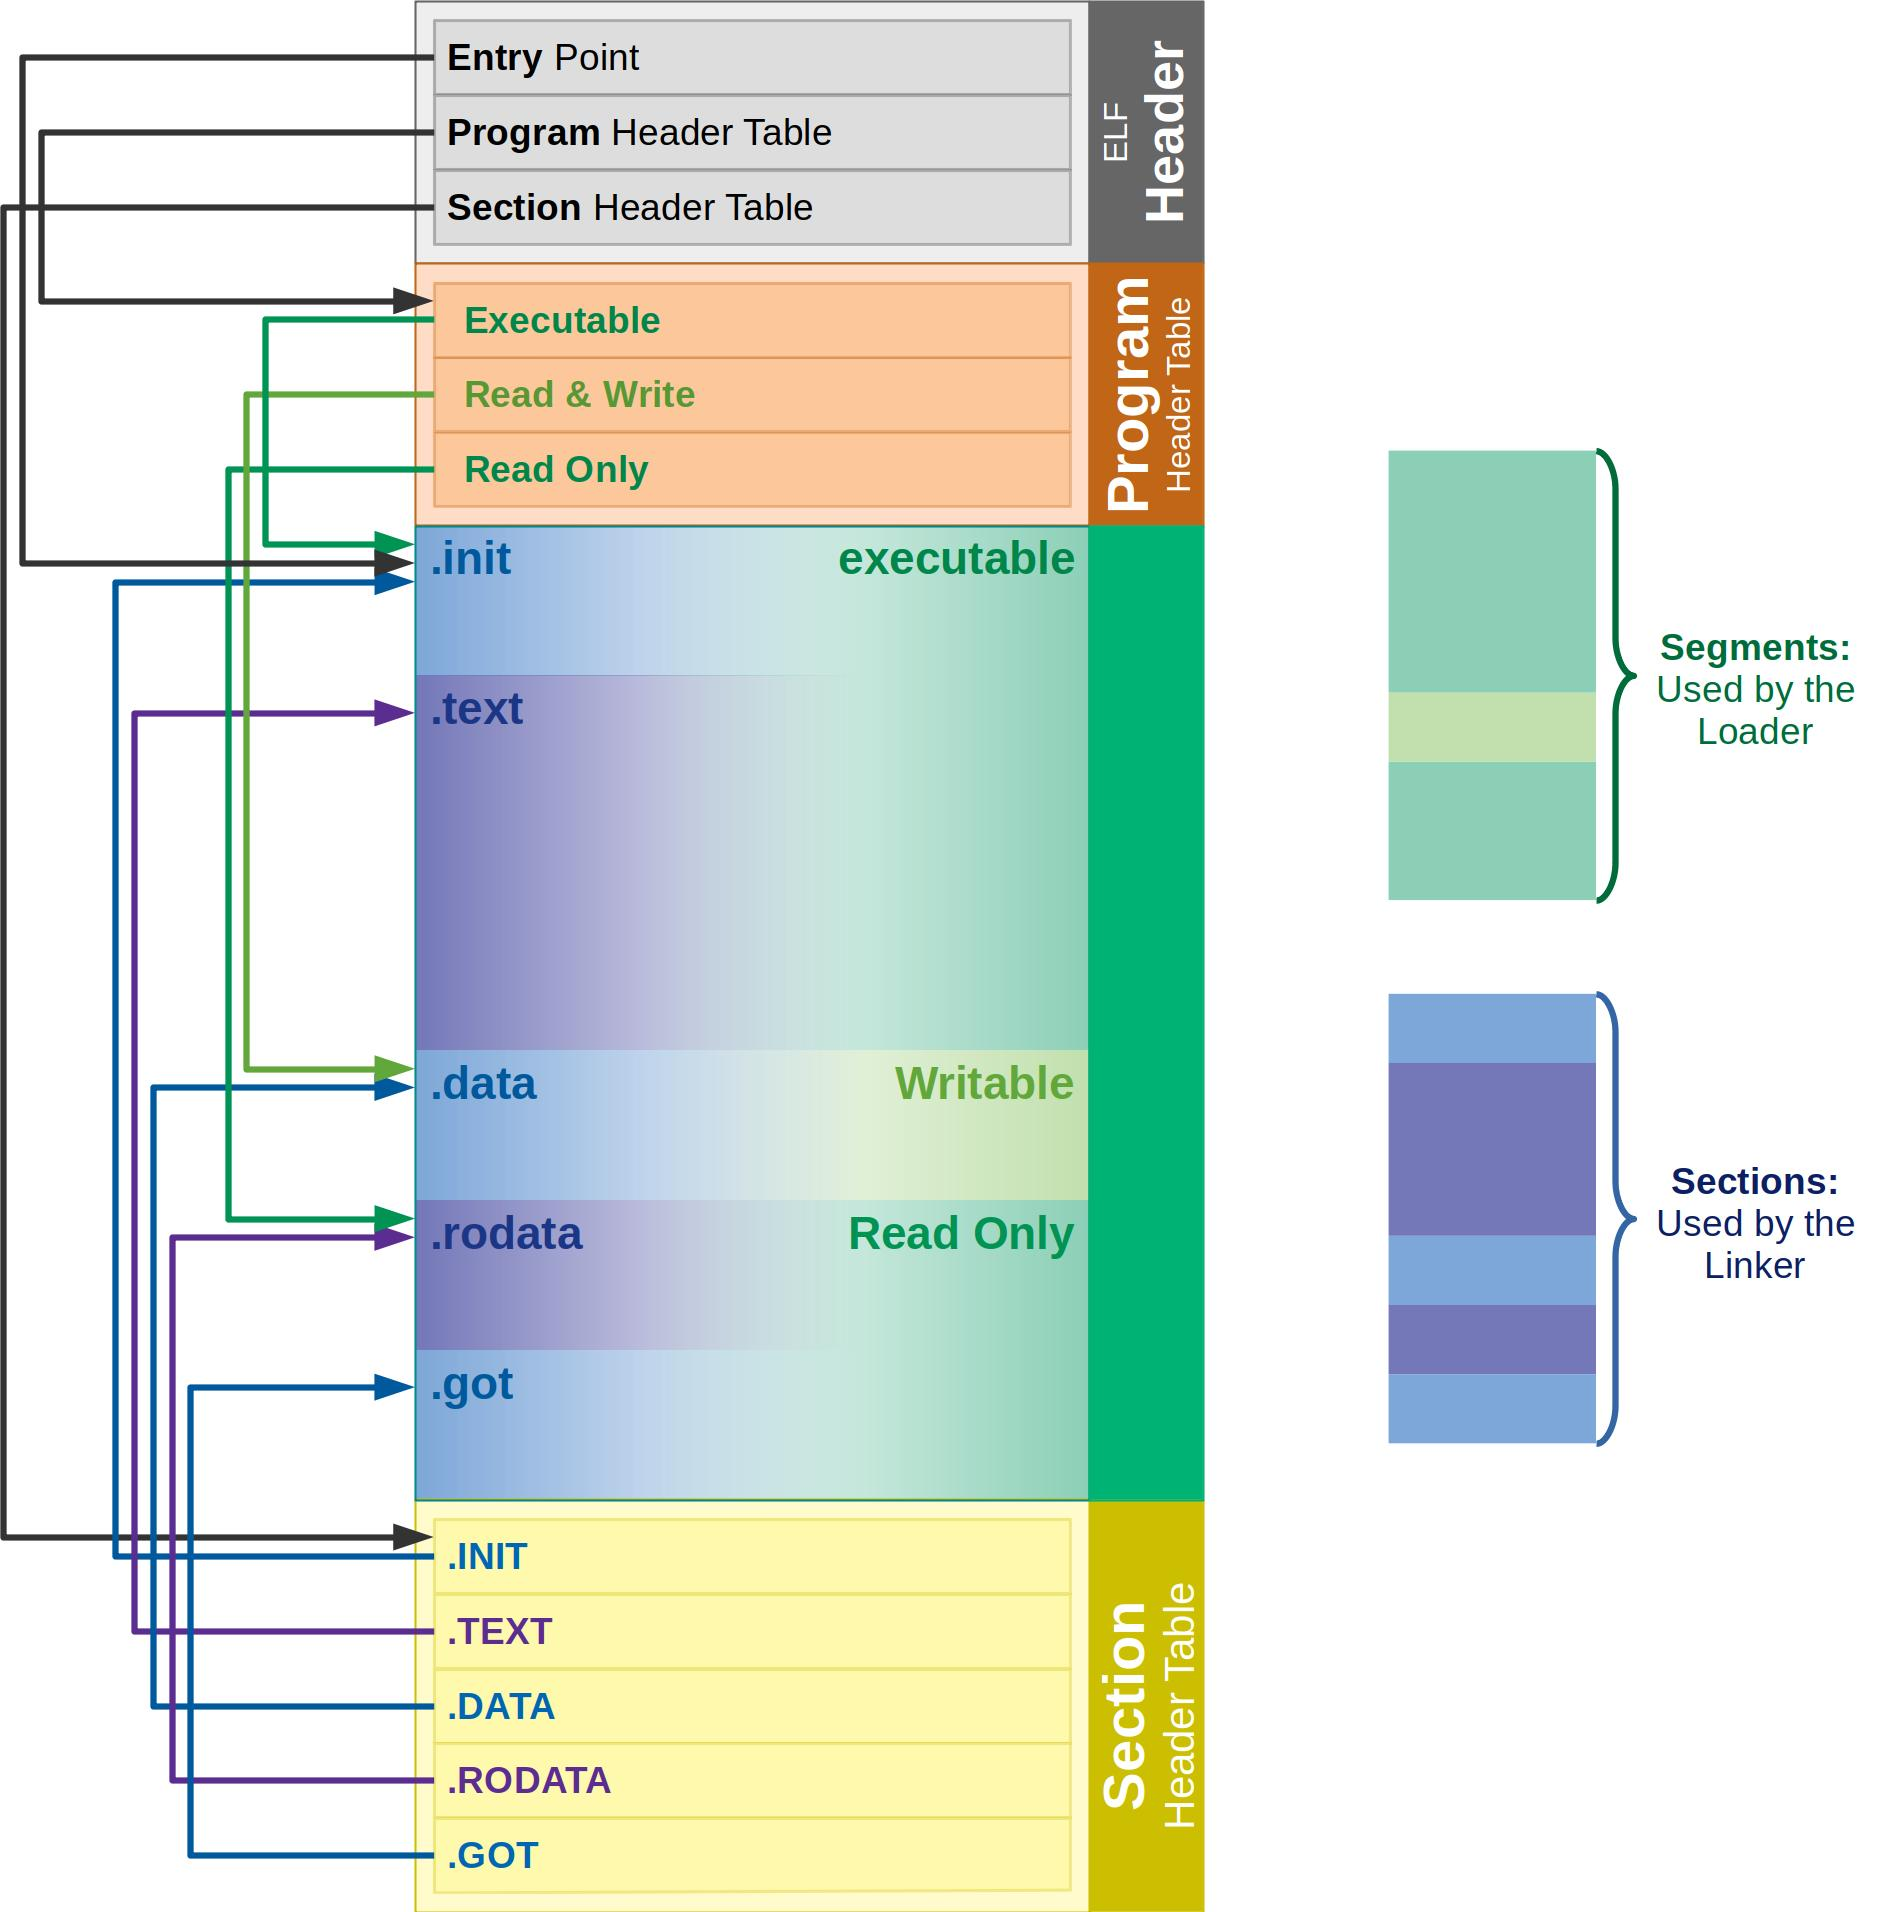
\includegraphics[width=300pt]{assets/typical_elf.jpg}
    \caption{Typical ELF file layout \cite{HW3238POperating}
    .}
    \label{fig:elf-layout}
\end{figure}


    \begin{minted}{text}
    $ fq .header /usr/bin/ls
        |00 01 02 03 04 05 06 07|01234567|.header{}:
    0x00|7f 45 4c 46 02 01 01 00|.ELF....|  ident{}:
    0x08|00 00 00 00 00 00 00 00|........|
    0x10|03 00                  |..      |  type: "dyn" (0x3)
    0x10|      3e 00            |  >.    |  machine: "x86_64" (0x3e)
    \end{minted}


An ELF file composed of a headers, which contains some
metadata about the file itself, segments containing the
actual code and some more metadata at the end. For the scope
of a package manager, it is of interest the study of this
data that is store on an ELF. It is also important to note
that there are two types of executable ELF's:

\begin{itemize}
    \item Statically linked executables
    \item Dynamically linked executables
\end{itemize}

Statically linked executable are usually not distributed by
Linux operating systems. A static executable bundles every
link-time dependency, such that everything is contained in a
single file. So from a distributor's point of view, it
doesn't make sense to make every file bundle every single
dependency, as they could be shared by other components of
the operating system. And some libraries even harder to
statically link, sometimes making it impossible in practice.

Dynamically linked executables and libraries, on the other
hand, rely on parts of the ELF metadata to be able to
discover other dependencies. When a executable is loaded,
via the |exec| system call, the following (non-exhaustive) steps are
performed by the kernel:

\begin{itemize}
    \item The kernel reds the \acl{PHT} which contains
    |INTERP|, this is the requested interpreter for the
    binary.
    \begin{minted}[breaklines]{text}
$ eu-readelf -l /usr/bin/ls
Program Headers:
  INTERP         0x000318 0x0000000000000318 0x0000000000000318 0x00001c 0x00001c R   0x1
        [Requesting program interpreter: /lib64/ld-linux-x86-64.so.2]
  ...
    \end{minted}
    \item Control is transfered to the loader, in this case
    |ld-linux-x86-64.so.2| .
    \item The loader then looks into a different section:
    the |.dynamic|
    \begin{minted}[breaklines]{text}
$ eu-readelf -d /usr/bin/ls
Dynamic segment contains 24 entries:
 Addr: 0x0000000000021a98  Offset: 0x020a98  Link to section: [ 7] '.dynstr'
  Type              Value
  NEEDED            Shared library: [libselinux.so.1]
  NEEDED            Shared library: [libc.so.6]
...
\end{minted}
    \item For each |NEEDED| library, the loader opens it and
    performs the symbol relocations to load them into
    memory.
    \item Finally, the control is transferred into the
    |_start| symbol, which performs some actions and then
    loads the |main| function for a C program.
\end{itemize}

This link loader (also known as dynamic linker) is part of
libc, one of the most important libraries in a Linux
operating system, that provides the standard C library. What
is important from the package manager's perspective, is how
ld-linux loads the dependencies for the |NEEDED| sections.
The manual page for |ld.so| \cite{LdLinuxManual} explains
the following behavior:

\begin{minted}[breaklines]{text}
If a shared object dependency does not contain a slash, then it
is searched for in the following order:

o  Using the directories specified in the DT_RPATH dynamic
   section attribute of the binary if present and DT_RUNPATH
   attribute does not exist.  Use of DT_RPATH is deprecated.

o  Using the environment variable LD_LIBRARY_PATH, unless the
   executable is being run in secure-execution mode (see below),
   in which case this variable is ignored.

o  Using the directories specified in the DT_RUNPATH dynamic
   section attribute of the binary if present.  Such directories
   are searched only to find those objects required by DT_NEEDED
   (direct dependencies) entries and do not apply to those
   objects' children, which must themselves have their own
   DT_RUNPATH entries.  This is unlike DT_RPATH, which is applied
   to searches for all children in the dependency tree.

o  From the cache file /etc/ld.so.cache, which contains a
   compiled list of candidate shared objects previously found in
   the augmented library path.  If, however, the binary was
   linked with the -z nodeflib linker option, shared objects in
   the default paths are skipped.  Shared objects installed in
   hardware capability directories (see below) are preferred to
   other shared objects.

o  In the default path /lib, and then /usr/lib.  (On some 64-bit
   architectures, the default paths for 64-bit shared objects are
   /lib64, and then /usr/lib64.)  If the binary was linked with
   the -z nodeflib linker option, this step is skipped.
\end{minted}

Usually for a conventional Linux distribution, the last
option is the most transversed. That is, loading file from
the default search path in |/usr/lib| or |/lib|. However,
for the software deployment model proposed in the previous
sections, packages don't link again the default search path,
as this causes the issues already explained.
|/etc/ld.so.cache| is also a shorthand for adding
globally-available libraries into the search path.

Finally, what the ELF format provides is the |RUNPATH|
section, which is searched for libaries contained in the
|NEEDED| sections. This |RUNPATH| is very useful, as it
allows every single binary file, to know where to look for
its own hashed dependencies. The link loader can also be
changed to a specific version, instead of relying in a
global |ld-linux.so|. This is done by changing the
|INTERP| in the \ac{PHT}.


As an alternative to a global search path such as the
following layout:

\begin{minted}{text}
INTERP   /lib/ld-linux.so.6
NEEDED   Shared library: [libc.so.6]
RUNPATH  -
\end{minted}

The following layout for an ELF file can be constructed:

\begin{minted}{text}
INTERP   /miq/store/libc-hashAAA/lib/ld-linux.so.6
NEEDED   Shared library: [libc.so.6]
RUNPATH  Library runpath: [/miq/store/libc-hashAAA/lib]
\end{minted}

With a modification of the ELF file metadata, then it is
possible to have a file load exactly the dependencies that
are computed at build time, to support the deployment model
discussed previously. The following chapter describes how
this modification of the ELF metadata is performed.

\FloatBarrier
\section{Other file types}

Not every file in a Linux system is an binary (ELF) file
however. A common Linux system is composed of many ``glue''
shell scripts, or any other text-based file. These files,
also perform the same ``dependency resolving'' that is done
in an ELF, but in a different way. For example, a shell
script that contains the following content:

\begin{minted}{sh}
#!/bin/sh

for file in /srv/backup/*; do
    cp $file /srv/backup2/
    chmod 600 /srv/backup2/$file
done
\end{minted}

A shell script like this also performes another type of
dependency resolution at run-time: loading any existing
program from |PATH|. In this case, both the |cp| and |chmod|
programs are external to the script, and also implicitely
dependencies of itself. For a toy script, it is easy to
underestimate this type of dependency resolution (as |cp|
and |chmod| are included in every Linux distribution), but
as scripts grow bigger, with more and more dependencies, it
becomes hard to keep track of every package.

The first line contains the |#!| sequence, which is called a
``shebang''. Analgous to the ELF format and |ld-linux|, the
shebang instruct Linux to load the program in this path, and
pass the rest of the file into it for execution. In turn
``sh'', interprets the rest of the file as a shell script,
and when faced with the |cp| and |chmod| commands, it reads
the environment variable |PATH|. This is also analogous to
the |RUNPATH| section of a ELF file, but contains
directories with executables:

\begin{minted}[breaklines]{text}
$ printenv PATH | tr ':' '\n'
/usr/local/sbin
/usr/local/bin
/usr/sbin
/usr/bin
/sbin
/bin
/usr/games
/usr/local/games
/usr/lib/wsl/lib
/snap/bin
\end{minted}

These folders are scanned sequentially, until the first
match is found -- that is |/usr/local/sbin/cp|, |/usr/local/bin/cp|, etc.

To avoid this kind of ``implicit'' dependency resolution,
one could also try to use the same technique used for ELF,
namely changing the |RUNPATH|. Unfortunately, this is not
possible, as scripts don't contain any extra ``metadata''
attached to them. A different solution is to construct a
shell script that contains full paths into the required
programs, and their full hashed paths in the store:

\begin{minted}{sh}
#!/miq/store/sh-version-hashAAA/bin/sh

for file in /srv/backup/*; do
    /miq/store/coreutils-version-hashAAA/bin/cp $file /srv/backup2/
    /miq/store/coreutils-version-hashAAA/bin/chmod 600 /srv/backup2/$file
done
\end{minted}

Doing these modifications is not as seamless as tweaking some
compile and link flags for an ELF file, and an automation
tool would be required to resolve the implicit dependencies
of a shell script.

The list of language-specific tweaks would continue -- for
example |PYTHONPATH| for Python packages -- but for the sake
of simplicity, only shell scripts and binary ELF files are
considered in this project. Usually each language ecosystem
has each own method of dependency resolution that can be
overriden to not use a ``global'' search path.

\FloatBarrier
\section{Base Linux packages}

To understand the scope of a Linux package manager, we need
to define what constitutes a Linux operating system. To
answer this question, we can take a look at the past, on the
inception on Linux. We can trace back to the UNIX system
\cite{ritchieUNIXSystemEvolution1984} developed by Ken
Thompson, Dennis Ritchie, and others. This operating system
marked a milestone in the history of computing, and the work
of its authors could be divided into 2 research fields: the
development of the interfaces of the OS, and a new
programming language to accompany it, the C programming
language. The UNIX kernel was rewritten in this new
language, and in 1978, the book
``The C Programming Language''
\cite{ritchieProgrammingLanguage1983} was
released, setting the foundation of the language into the
future. As UNIX started to gain popularity, the project
increasingly started to lock users in. As an alternative to
UNIX, the GNU (GNU is Not Unix) project started with the
intention to provide a UNIX-compatible operating system that
would not lock users in with proprietary software licenses.
Finally, the Linux kernel was created by Linus Torvalds
around 1991 as a research project to provide a substitute to
the MINIX kernel, and finally the GNU components replaced
any leftovers of MINIX \cite{OverviewGNUSystem}.

The Linux kernel and all of the GNU components were written
in C, so it became the de-facto language for system
software. Therefore, the C language is intertwined with how
a Linux operating system works, and all the packages that
compose it from the kernel to userland. From the packager's
perspective, there is one package that is the most
important: \textbf{libc}. The C standard library (libc, or
GNU's libc implementation, glibc) is a collection of C
headers and library objects that provide interfaces to the
operating system for programs written in C. Libc was
standardized in 1999 by the ISO C committee under the C99
language specification, and further revisions were made to
update it. Some of the headers from libc include:

\begin{figure}[hbt]
    \centerfloat
    \begin{tblr}{hlines, vlines}

        <string.h> & String manipulation \\

        <stdio.h> & Standard input/output \\

        <stdint.h> & Standard integer types \\

        ... & ... \\

    \end{tblr}
    \caption{Some of the headers from libc.}
\end{figure}

For Linux, there are various implementations of libc, such
GNU's glibc or musl libc \cite{MuslLibc}, being the former
the predominant on all popular Linux distributions. Along
with the headers required by the C ISO standard, the libc
providers are implemented over the kernel's system calls and
also provide UNIX-specific interfaces, namely |<unistd.h>|.
Libc is also the provider of the link-loader discussed in
previous sections (ld-linux.so), and also injects some
loading code in every ELF file, before the main function
execution takes over.

Apart from libc, many programs and libraries are implemented
on top of it, to provide what is called as the \acl{LSB}
\cite{LinuxStandardBase} . This specification outlines some
of the most important programs that compose a Linux system,
such as ``coreutils'', which contains the most basic
terminal utilities, like |ls|, |cat|, |cp|, etc. To be able
to build the components, it is also needed a C compiler,
which is also provided by the GNU project in form of GCC
(GNU Compiler Collection). To
be able to support the compilation and configuration of
programs, some other tools are required like |make| or
|sed|, and also a POSIX shell to interact with the system,
in the form of |bash|. The table \ref{tab:lsb} outlines some
of these componentes and their functionality.

\begin{figure}[hbt]
    \centerfloat
    \begin{tblr}{hlines, vlines}
        libc & C standard library (glibc, musl) \\

        gcc & C and C++ compiler \\
        coreutils & Basic terminal utilities, like ls,
        cat, cp, etc. \\
        binutils & Binary utilities, like ld, as,
        objdump, etc. \\
         make & Build automation tool \\
         sed & Stream editor, text modification
        program \\
         bash & POSIX shell implementation \\
         tar & Archive utility \\
         grep & Text search utility \\
         findutils & File search utilities, like
        find or findmnt \\
         diffutils & File comparison utilities, like
        diff \\
         systemd & System and service manager \\
    \end{tblr}
    \caption{Some of the basic components of a Linux system.}
    \label{tab:lsb}
\end{figure}

As a Linux distribution grows in scope, more and more
components are needed to build something that an end-user is
able to use. Starting from graphical toolkits, like GTK or
QT, to the X11 display server and desktop environments, like
Gnome or KDE Plasma. And every component in-between, like
proper service management via systemd, the package manager
itself, network management, power management, peripherals
support, and all the libraries that are required to build
all the ``leaf'' packages of the full dependency tree.
Finally, the kernel itself is also a package with special
properties (as it doesn't depend on libc), but regardless of
importance.

The scope of this work has been limited to a basic terminal
usage of Linux packages, so the focus won't be on building
complex software, but rather building basic components to
prove the viability of the deployment model. It is also
important to note, that while packages can be put together
to form a fully function independent operating system, a
package manager of Linux packages can work as a ``guest'' on
a different distribution. This is, running Linux packages
that are not part of the distribution itself. For a
classical system, this has never been common practice -- for
example, installing apt (Debian's package manager) on a
Gentoo system -- mainly limited by the rules imposed by the
\acl{FHS}. Basically, two package managers would interfere
with each other, as they would try to manage files that were
managed by the other package manager (any file on /usr/bin,
/usr/lib, etc). However, with the usage of the special
hash-based paths, this problem not an issue, as miq can be
used on top of any Linux distribution, without interfering
with it.

\FloatBarrier
\section{The bootstrapping problem}

As discussed in the previous section, the scope of this work
is to be able to demonstrate the viability of the deployment
model of hashed paths instead of relying in the \ac{FHS}.
So, as one of the core libraries, libc is the one to be
compiled the first. As mentioned previously, libc is the C
standard library, that in practice is used by every program
written in C, which make up the core programs of a Linux
operating system. To be able to compile libc, it is required
a C compiler (from GCC), a POSIX shell (bash, for
example) and other utilities. In this project, musl libc was used instead of
glibc, as GNU's version contains some extra additions that
are not part of the standard, which could introduce
complexity. Then, a dependency graph for musl libc can be
drawn as shown in figure \ref{fig:libc-deps}.

\begin{figure}[hbt]
    \centerfloat
    \includesvg[width=150pt]{graph/libc-bs1.dot.svg}
    \caption{Dependency graph for musl libc on first iteration.}
    \label{fig:libc-deps}
\end{figure}

These GCC dependency in this graph is assumed to already
"exist" in the system. But as already discussed, this is a
source of impurity, as we don't know what C compiler was
used, we can't hash the input to produce a hash for the musl
output. This C compiler is ``external'' to the system.
Therefore one of the objectives of any package manager is to
be able to ``support'' itself, to be able to produce
packages without any external interference. Then, this GCC
must come from the package manager itself as well, and we
can draw its dependency graph in figure \ref{fig:libc-deps2} .

\begin{figure}[hbt]
    \centerfloat
    \includesvg[width=200pt]{graph/libc-bs2.dot.svg}
    \caption{Dependency graph for musl libc on second iteration, recursive nature shows.}
    \label{fig:libc-deps2}
\end{figure}

As can be seen, to be able to build libc, we need a C
compiler, and to build a C compiler we need libc. This is a
problem of a circular dependency, in particular the
bootstrapping problem, because we need to ``base'' to be
able to lift the entire system system from the ground.
Moreover, if we try to draw a dependency from cyclically as
in figure \ref{fig:libc-deps3}, we can see that graph is now
\emph{cyclic}, this means that it is no longer a \ac{DAG} as
discussed in the previous section, and we can no longer hash
the nodes, as it would result in a infinite recursion. For
this reason, cyclic dependencies are not allowed in miq, and
using and checking for a proper \ac{DAG} is important.

\begin{figure}[hbt]
    \centerfloat
    \includesvg[width=150pt]{graph/libc-bs3.dot.svg}
    \caption{Cyclic dependency graph for musl libc and gcc.}
    \label{fig:libc-deps3}
\end{figure}

To solve the bootstrapping problem, a solution is proposed
of providing a set of bootstrap tools. This set of tools is
downloaded from the internet, ready to use. By using it as a
``fixed hash'' package, we can break the chain of recursive
dependencies, as shown in figure \ref{fig:libc-deps4}. This
set of bootstrap tools doesn't need to be updated ever. For
example, they could contain a very old GCC, such that it is
recent enough to be able to compile a newer GCC used for the
rest of the packages on the system.

\begin{figure}[hbt]
    \centerfloat
    \includesvg[width=150pt]{graph/libc-bs4.dot.svg}
    \caption{Dependency graph for musl libc with a loop on gcc, solved with a bootstrap package.}
    \label{fig:libc-deps4}
\end{figure}

In practice, the Linux distributions don't use the first
iteration of this process. Instead, an iterative process is
created, where libc and the C compiler (along any extra
tools) are compiled in succession, using the result of the
previous step to compile the next one. These are called
``stages'', and the process ``distills'' the programs until
an stable result is obtained. The final stage (from 0 to 1,
2 , etc) is then used to build the system, instead of the
zero-th stage.

\begin{figure}[hbt]
    \centerfloat
    \includesvg[width=200pt]{graph/libc-bs5.dot.svg}
    \caption{Bootstrap tower with 3 stages.}
    \label{fig:libc-deps5}
\end{figure}


\section{GNU Autotools}

\FloatBarrier
\chapter{Implementation}

\section{Dependency solver}

\section{Recipe evaluator}

\section{Builder}


\section{Database}


